\section{Hardware}
Celá platforma se skládá z jednoho řídicího prvku (viz. kapitola \ref{sec:HWserver}) a třech (maximální počet klientů je hardwarově limitován na čtyři) klientských zařízení (viz. kapitola \ref{sec:HWclient}). Datové spojení je realizováno hvězdicovou topologií (schéma na obrázku \ref{fig:schema_net}). Jako centrální prvek byl použit switch D-Link DGS-105.
Celá demonstrační sestava se pak skládá z:
\begin{itemize}
  \item 1x switch D-Link DGS-105
  \item 1x server s Arduino DUE
  \item 3x klient s Arduino Ethernet a dotykovým displejem
  \item 4x propojuvací UTP kabel
  \item 1x napájecí adaptér pro switch (5 V/1 A součástí balení)
  \item 4x napájecí adaptér 12 V/1500 mA
\end{itemize}

\begin{figure}[hbtp]
  \centering
  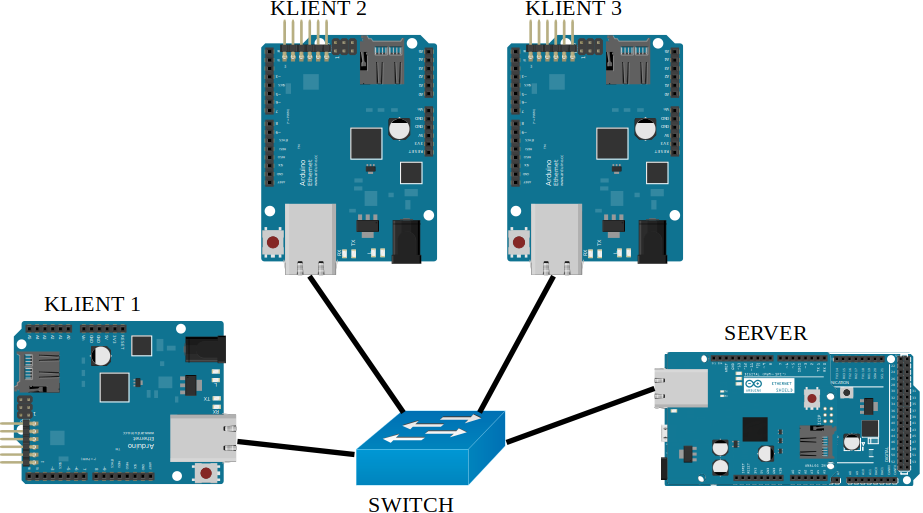
\includegraphics[width=12cm]{img/schema_net.png}
  \caption{\label{fig:schema_net} Schéma zapojení jednotlivých zařízení do sítě, zdroj \cite{fig_ArdEthernet, fig_ArdEthShield, fig_switchIco, fig_ArdDue}}
\end{figure}

\subsection{Zařízení typu server}
\label{sec:HWserver}
Zařízení je založeno na desce \textit{Arduino Due}, které obsahuje mikrokontrolér Atmel SAM3X8E ARM Cortex-M3 s 512 kB flash paměti a nabízí dostatečný výkon pro správné fungování serveru. Původní varianta totiž počítala s nasazením desky \textit{Arduino Ethernet} i jako serveru. To se ovšem vzhledem k omezeným prostředkům ukázalo jako problematické, proto byla zvolena právě deska \textit{Arduino Due}.

Pro připojení do sítě je použit Ethernetový shield s čipem Wiznet W5100, který je přímo napojen na Arduino. Tímto je dána ona limitace maximálně na 4 hráče, protože dle datasheetu výrobce čipu \cite{datasheet_w5100} je maximální počet spojení právě čtyři.

Pro pohodlné ovládání jsou k serveru připojena dvě tlačítka a jedna barevná svítivá dioda. Význam jednotlivých stavů svítivé diody a funkce tlačítek je popsána v kapitole \ref{sec:ovladani}. Propojení těchto periferií s Arduinem je realizováno pomocí jednostrané DPS, schéma zapojení je pak na obrázku \ref{fig:server_module}.

\begin{figure}[hbtp]
  \centering
  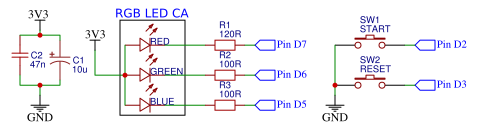
\includegraphics[width=12cm]{img/server_module.png}
  \caption{\label{fig:server_module} Schéma zapojení periferií u serveru}
\end{figure}

Napájení je řešeno externím adaptérem, dle stránek výrobce \cite{ArdDue_web} je možné pužít napětí 6 - 16 V (využívá se interní stabilizátor), přižemž odběr je kolem 140 mA při napájení 12 V. V případě, že je pro ovládání použita sériová linka (server je připojen USB kabelem k počítači, ovládání tímto způsobem je popsáno v kapitole \ref{sec:ovladani}), postačuje napájení dodané přes USB kabel a není potřeba připojovat externí napájecí zdroj.

Celé zařízení je pak umístěno v krabičce jejíž návrh je na obrázku \ref{fig:server_navrh} a realizace na obrázku \ref{fig:server_realizace}. Krabička byla navrhnuta v programu Autodesk Inventor Professional 2019 Student Edition a realizovaná 3D tiskem na tiskárně Original Prusa i3 MK3S. Krabička je osazena červeným a zeleným tlačítkem, barevnou sívitvou 5~mm diodou (se společnou anodou) a souosým napájecím konektorem 5,5x2,1~mm. Pro upevnění Arduina jsou použity šrouby M2,5x10 a závitové vložky M2,5x6 vtavené do připravených otvorů v krabičce. Arduino deska sice nabízí montážní otvory o průměru 3~mm, ale vzhledem k rozložení součástek zde není dostatek místa pro hlavu šroubu~M3.

\begin{figure}[hbtp]
\centering
\begin{minipage}[c]{\textwidth/2-1cm}
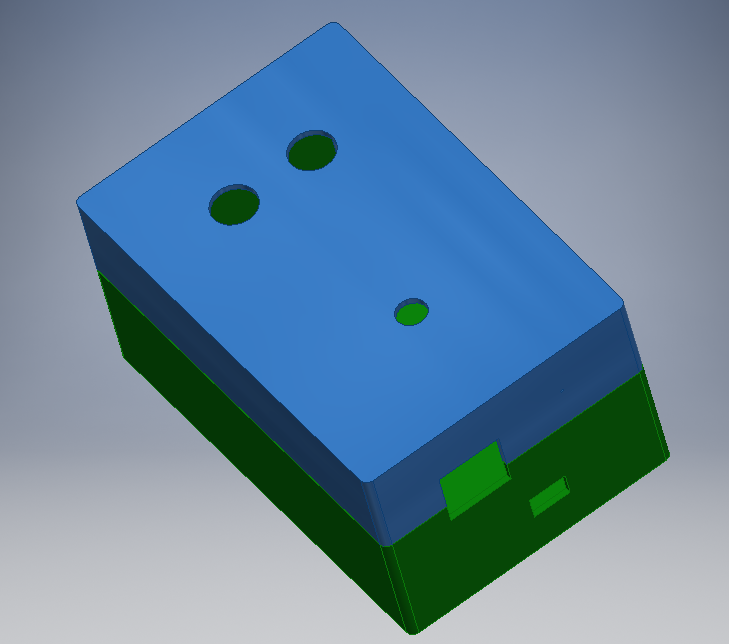
\includegraphics[width=\textwidth]{img/foto/server_navrh.png}
\end{minipage}
\begin{minipage}[c]{\textwidth/2-1cm}

\includegraphics[width=\textwidth]{img/foto/server_realizace.png}
\end{minipage}
\\
\begin{minipage}[c]{\textwidth/2-0.5cm}
\caption{\label{fig:server_navrh}Návrh krabičky pro server}
\end{minipage}
\begin{minipage}[c]{\textwidth/2-.5cm}
\caption{\label{fig:server_realizace}Zkompletovaná krabička pro server}
\end{minipage}
\end{figure}


\subsection{Zařízení typu klient}
\label{sec:HWclient}
Zařízení je založeno na desce Arduino Ethernet, která je vybavena mikrokontrolérem ATmega328 s 32 kB flash paměti. Tato deska byla zvolena především kvůli tomu, že má vestavěný ethernetový kontrolér, který tak nezabírá piny pro připojení shieldu s displejem. Malá flash paměť se však během vývoje ukázala jako značně limitující, protože při nahrání všech potřebných knihoven (popsáno v kapitole~\ref{sec:knihovny}) zůstalo k dispozici 30~\% programové paměti. I z tohoto důvodu byla zvolena jako hra piškvorky, která není programově příliš složitá a také bylo nutné vynechat složitější menu například s nastavením barvy nebo změny IP adresy serveru (to se nyní musí provádět změnou v kódu a přeprogramováním Arduina, více v kapitole \ref{sec:client-nastaveni}).

Jak už bylo zméněno výše, tato deska má věstavěný ethernet kontrolér WIZnet W5100. U klienta není maximální počet spojení limitující (klient drží pouze jedno spojení se serverem), jedinou nevýhodou kontroléru W5100 tak zůstává, že neobsahuje registr, ve kterém je uložena informace o fyzickém připojení ethernetového kabelu k desce \cite{datasheet_w5100}. Tím je zkomplikována detekce připojení a odpojení kabelu.

Pro interakci s uživatelem je klient vybaven 2,4" barevným TFT LCD displej s rozlišením 320x240 pixelů s rezistivní dotykovou plochou. Displej je vybaven  řadičem SUM74HC245T. Vzhledem k rozměrům (výšce) RJ-45 konektoru, který je umístěn na desce, je nutné pro správné připojení použít lištu oboustrannými kolíky o délce kolíku minimálně 15~mm. Protože u displejů použitých v tomto projektu byly kolíky připájeny už od výrobce, byla dodatečně vyrobená patice s dutinkové lišty a lišty s oboustrannými kolíky.

Pro napájení byl zvolen externí napájecí adaptér, avšak připojení na integrovaný stabilizátor není možné, protože displej při 5~V odebírá přibližně 400~mA, což integrovaný stabilizátor nedokáže poskytnout (vlivem velého ztrátového výkonu dochází k jeho značnému zahřívání). Napájení přímo napětím 5~V není také příliš vhodné, protože vlivem například ztrát přívodních vodičů může dojít ke kolísání napětí, tím dojde i k pohybu reference AD převodníku připojenému k dotykové vrstvě displeje a tak může docházet k nesprávnému vyhodnocení stisku (může se lišit reálné místo stisku od toh, které vyhodnotil mikrokontrolér). Jako nejlepší varianta se ukázalo použití modulu se snižujícím DC-DC měničem. Modul obsahuje spínací regulátor MP1584 a dle dodavatele je schopen pracovat s napětím 6~-~25~V (při výstupním napětí 5~V) a dodat proud až 1,5~A, což je pro tuto aplikaci dostačující.

Stejně jako v případě serveru je celé zařízení umístěno ve vytištěné krabičce, návrh a realizovaná krabička jsou na obrázcích \ref{fig:client_navrh}, \ref{fig:client_realizace}. Princpi uchycení Arduina je stejný jako v případě serveru, pro napájení je opět osazen souosý napájecí konektor 5,5x2,1~mm. Dále je z boku výřez por konektor RJ-45 pro připojení do ethernetové sítě a na vrchu se nachází výřez pro displej vedle kterého se je umístěn otvor pro přístup k resetovacímu tlačítku.

\begin{figure}[hbtp]
\centering
\begin{minipage}[c]{\textwidth/2-1cm}
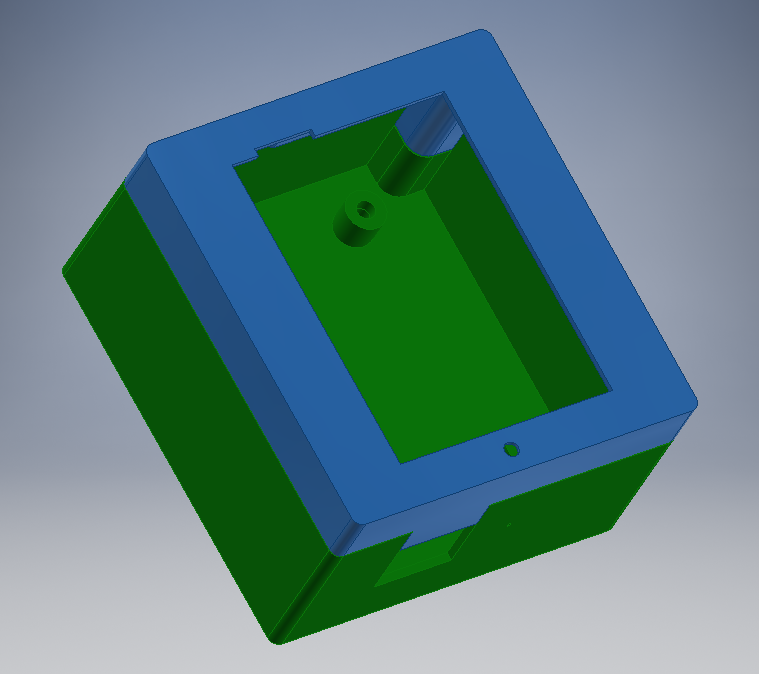
\includegraphics[width=\textwidth]{img/foto/client_navrh.png}
\end{minipage}
\begin{minipage}[c]{\textwidth/2-1cm}

\includegraphics[width=\textwidth]{img/foto/client_realizace.png}
\end{minipage}
\\
\begin{minipage}[c]{\textwidth/2-0.5cm}
\caption{\label{fig:client_navrh}Návrh krabičky pro klienta}
\end{minipage}
\begin{minipage}[c]{\textwidth/2-.5cm}
\caption{\label{fig:client_realizace}Zkompletovaná krabička pro klienta}
\end{minipage}
\end{figure}
